\chapter{Reconstrucci\'on Geom\'etrica e Inferencia Homol\'ogica}

Otra forma de construir cubiertas y usar sus nervios para exhibir la estructura topol\'ogica de los datos
es considerar la uni\'on de bolas centradas en los puntos de los datos. En esta secci\'on suponemos que
$\mathbb{X}_n = \left\{x_0, \dots, x_n\right\}$ es un subconjunto de $\mathbb{R}^{d}$, muestrado de manera
i. i. d. de acuerdo con la medida de probabilidad $\mu$ con soporte compacto $M\subset\mathbb{R}^{d}$. La
estrategia general para inferir informaci\'on topol\'ogica acerca de $M$ a trav\'es de $\mu$ consiste en
dos pasos:

\begin{enumerate}
    \item Se cubre $\mathbb{X}_{n}$ con una uni\'on de bolas de radio fijo con centros en las $x_{i}$'s.
    Bajo algunas condiciones de regularidad en $M$, se puede relacionar la topolog\'ia de esta uni\'on de
    bolas con la de $M$.
    
    \item Desde un una perspectiva pr\'actica y algor\'itmica, las cualidades topol\'ogicas de $M$ son
    inferidas del nervio de la uni\'on de las bolas, utilizando el teorema del nervio.
    
\end{enumerate}

De esta manera, es posible comparar espacios a trav\'es de equivalencias isot\'opicas, una noci\'on m\'as
fuerte que la de homeomorfismo: $X\subseteq\mathbb{X}^{d}$ y $Y\subseteq\mathbb{X}^{d}$ se dicen ser
(ambientalmente) isot\'opicos si existe una familia continua de homeomorfismos
$H: \left[0, 1\right]\times\mathbb{R}^{d}\rightarrow\mathbb{R}^{d}$, $H$ continua, tal que, para cualquier
$t\in\left[0, 1\right]$, $H_{t} = H\left(t, \cdot\right):\mathbb{R}^{d}\rightarrow\mathbb{R}^{d}$ es un
homeomorfismo, $H_{0}$ es el mapeo identidad en $\mathbb{R}^{d}$, y $H_{1}\left(X\right)=Y$.
Es claro que, si $X$ y $Y$ son isot\'opicos, entonces son homeomorfos. El rec\'iproco no es cierto:
un c\'irculo anudado y uno desanudado en $\mathbb{R}^{3}$ son homeomorfos pero no isot\'opicos.

\section*{Funciones DL y Reconstrucci\'on}

Dado un suconjunto compacto $K\subset\mathbb{R}^{d}$ y un n\'umero real no negativo $r$, la uni\'on de
bolas de radio $r$ centradas en $K$, $K^{r} = \cup_{x\in K}B\left(x, r\right)$, llamado el
$r$-cubrimiento de $K$, es el conjunto de $r$-subnivel de la distancia
$d_{K}:\mathbb{R}^{d}\rightarrow\mathbb{R}$ definida por
$d_{K}\left(x\right) = \inf_{y\in K}\left\|x-y\right\|$; es decir,
$K^{r} = d^{-1}_{k}\left(\left[0, r\right]\right)$. Esto nos permite utilizar propiedades diferenciales
de funciones distancia y nos ayuda a comparar la topolog\'ia de los cubrimientos de conjuntos compactos
 que est\'en cercas el uno del otro con respecto a la distancia de Hausdorff.
 
\begin{definicion}
    (Distancia de Hausdorff en $\mathbb{R}^{3}$). La distancia de Hausdorff entre dos subconjuntos compactos
    $K$, $K'$ de $\mathbb{R}^{d}$ esta definida como
    \begin{equation*}
        d_{H}\left(K, K'\right) = \left\|d_{K}-d_{K'}\right\|_{\infty} =
        \inf_{x\in\mathbb{R}^{d}}\left|d_{K}\left(x\right)-d_{K'}\left(x\right)\right|
    \end{equation*}
\end{definicion}
 
Aqu\'i, los conjuntos compactos son el conjunto de datos $\mathbb{X}_{n}$ y el soporte $M$ de la
medida $\mu$. Cuando $M$ es una subvariedad compacta suave, bajo ciertas condiciones sobre
$d_{H}\left(\mathbb{X}_{n}, M\right)$, para alg\'un $r$ bien escogido, las coberturas de
$\mathbb{X}_{n}$ son homot\'opicamente equivalentes a $M$, Chazal y Lieutier (2008) \cite{Chazal2008},
Niyogi et al. (2008) \cite{Niyogi2008} (Ver Figura \ref{fig:Figura 5}). Estos resultados se extienden
a clases m\'as grandes de conjuntos compactos y llevan a resultados fuertes sobre inferencia de los
tipos de isotop\'ias de las coberturas de $M$, Chazal et al. (2009c) \cite{Chazal2009c},
Chazal et al. (2009d)\cite{Chazal2009d}. Tambi\'en llevan a resultados en la estimaci\'on de otras
cantidades geom\'etricas y diferenciales tales como normales, Chazal et al. (2009c) \cite{Chazal2009c},
curvaturas Chazal et al. (2009e) \cite{Chazal2009e}, o medidas de frontera,
Chazal et al. (2010) \cite{Chazal2010} bajo ciertas condiciones en la distancia de Hausdorff entre la
forma subyacente y los datos muestrales.
 
Estos resultados dependen de la $1$-semiconcavidad del cuadrado de la funci\'on distancia $d_{K}^{2}$,
esto es, la convexidad de la funci\'on $x\rightarrow\left\|x\right\|^{2}-d_{K}^{2}\left(x\right)$,
definida de a continuaci\'on.
 
\begin{definicion}
    Una funci\'on $\phi:\mathbb{R}^{d}\rightarrow\mathbb{R}_{+}$ es DL (distance-like) si es propia (la
    preimagen de cualquier conjunto compacto en $\mathbb{R}$ bajo $\phi$ es un compacto en
    $\mathbb{R}^{d}$) y $x\rightarrow\left\|x\right\|^{2}-\phi^{2}\left(x\right)$ es convexa.
\end{definicion}
 
Gracias a su semiconcavidad, una funci\'on DL $\phi$ tiene un gradiente
$\nabla\phi:\mathbb{R}^{d}\rightarrow\mathbb{R}^{d}$ bien definido, pero no continuo, que puede ser
integrado en un flujo continuo (Petrunin, 2007 \cite{Petrunin2007}) que permite rastrear la evoluci\'on
de la topolog\'ia de sus subniveles y compararla a una de los subniveles de funciones DL cercanas.
 
\begin{definicion}
    Sea $\phi$ una funci\'on DL y sea $\phi^{r}=\phi^{-1}\left(\left[0,r\right]\right)$ el $r$-subnivel
    de $\phi$.
    
    \begin{itemize}
        \item Un punto $x\in\mathbb{R}^{d}$ es llamado $\alpha$-cr\'itico si
        $\left\|\nabla_{x}\phi\right\|\leq\alpha$. El valor $r=\phi\left(x\right)$ correspondiente,
        tambi\'en es llamado $\alpha$-cr\'itico.
        
        \item El tama\~{n}o del atributo d\'ebil de $\phi$ en $r$ es el m\'inimo $r>0$ tal que $\phi$
        no tiene ning\'un valor cr\'itico entre $r$ y $r+r'$. Lo denotamos por
        $\mathrm{wfs}_{\phi}\left(r\right)$ (weak feature size). Para cualquier $0<\alpha<1$, el 
        $\alpha$-alcance de $\phi$ es el m\'aximo $r$ tal que $\phi^{-1}\left(\left(0,r\right]\right)$
        no contiene ning\'un punto $\alpha$-cr\'itico.
        
    \end{itemize}
\end{definicion}
 
El tama\~{n}o del atributo d\'ebil $\mathrm{wfs}_{\phi}\left(r\right)$ (respecto al $\alpha$-alcance)
mide la regularidad de $\phi$ sobre sus $r$-niveles (respecto al $O$-nivel). Cuando $\phi=d_{K}$ es
la funci\'on distancia a un conjunto compacto $K\subset\mathbb{R}^{d}$, el $1$-alcance coincide con el
alcance cl\'asico de la teor\'ia de la medida gem\'etrica, Federer (1959) \cite{Federer1959}. Su
estimaci\'on desde muestras aleatorias fue estudiada en Aamari et al. (2019) \cite{Aamari2019}. Una
propiedad importante de una funci\'on DL $\phi$ es que la topolog\'ia de sus subniveles $\phi^{r}$
s\'olo puede cambiar cuando $r$ cruza un valor $0$-cr\'itico.

\begin{lema}
    (Lema de isotop\'ia). Sea $\phi$ una funci\'on DL y $r_{1}<r_{2}$ dos n\'umeros positivos tales que
    $\phi$ no tiene puntos $0$-cr\'iticos, esto es, puntos $x$ tales que $\nabla\phi\left(x\right)=0$,
    en el subconjunto $\phi^{-1}\left(\left[r_{1},r_{2}\right]\right)$. Entonces todos los subniveles
    $\phi^{-1}\left(\left[0,r\right]\right)$ son isot\'opicos para $r\in\left[r_{1},r_{2}\right]$.
\end{lema}

\begin{figure}[ht]
    \centering
    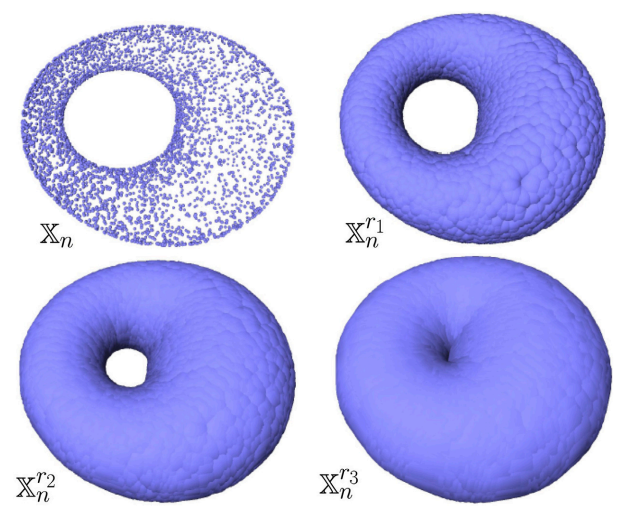
\includegraphics[width=0.85\linewidth]{./figures/Figura5.png}
    \caption{
        Ejemplo de una nube de puntos $\mathbb{X}_{n}$ muestreada en la
        superficie de un toro en $\mathbb{R}^{3}$ y sus coberturas para
        diferentes valores del radio $r_{1}<r_{2}<r_{3}$. Para valores
        bien escogidos del radio (por ejemplo $r_{1}$ y $r_{2}$), las
        coberturas son homot\'opicamente equivalentes al toro.
    }
    \label{fig:Figura 5}
    \vspace{15pt}
\end{figure}

Como consecuencia inmediata del lema de isotop\'ia, todos los subniveles de $\phi$ entre $r$ y
$r + \mathrm{wfs}_{\phi}\left(r\right)$ tienen la misma topolog\'ia. Ahora, el siguiente teorema de
Chazal et al. \cite{Chazal2011b}, proporciona una conexi\'on entre la topolog\'ia de los subniveles
de funciones DL cercanas.

\newpage

\begin{teorema}[Teorema de reconstrucci\'on]\label{teoRecon}
    Sean $\phi$, $\psi$ dos funciones DL, tales que
    $\left\|\phi-\psi\right\|_{\infty}\leq\epsilon$, con $\alpha$-alcance
    $\mathrm{reach}_{\alpha}\left(\phi\right)\geq R$ para algunos $\epsilon$ y $\alpha$ positivos.
    Entonces, para todo $r\in\left[4\epsilon/\alpha^{2}, R-3\epsilon\right]$ y cada
    $\eta\in\left(0, R\right)$ los subniveles $\psi^{r}$ y $\phi^{\eta}$ son homot\'opicamente
    equivalentes si:
    
    \begin{equation*}
        \epsilon\leq\frac{R}{5+4/\alpha^{2}}
    \end{equation*}
\end{teorema}

Bajo condiciones similares pero ligeramente m\'as t\'ecnicas, el teorema de reconstrucci\'on puede ser
extendido para probar que los subniveles son homeomorfos e incluso isot\'opicos
(Chazal et al., 2009 \cite{Chazal2009c}; Chazal et al., 2008 \cite{Chazal2008}).

Consideremos una vez m\'as $\phi = d_{M}$ y $\psi = d_{\mathbb{X}_{n}}$ las funciones distancia
al soporte de $M$ de la medida $\mu$ y al conjunto de puntos asociados a los datos $\mathbb{X}_{n}$,
la condici\'on $\mathrm{wfs}_{\alpha}\left(d_{M}\right)\geq R$ puede ser interpretada como una
condici\'on de regularidad sobre $M$\footnote{Por ejemplo, si $M$ es una subvariedad compacta suave,
el $0$-alcance $\mathrm{reach}_{0}\left(\phi\right)$ siempre es positivo se le llama el alcance de
$M$ Federer (1959) \cite{Federer1959}}. El teorema de reconstrucci\'on junto con el teorema del nervio
nos indican que para ciertos valores de $r$, $\eta$ y los $\eta$-cobertura son homot\'opicamente
equivalentes al nervio de la uni\'on de las bolas de radio $r$ centradas en $\mathbb{X}_{n}$, es decir,
el complejo de \v Cech $Cech_{r}\left(\mathbb{X}_{n}\right)$.

Desde un punto de vista estad\'istico, la principal ventaja de estos resultados sobre la distancia de
Hausdorff es que el problema de estimaci\'on de cantidades topol\'ogicas se transforma en una serie
de preguntas acerca de el soporte de ciertas medidas, las cuales han sido ampliamente estudiadas.

\section{Inferencia Homol\'ogica}

Los resultados anteriores proporcionan una estructura matem\'atica bien fundamentada para inferir la
topolog\'ia de las formas de un complejo simplicial construido sobre una muestra finita que sirve como
aproximaci\'on. Sin embargo, desde una perspectiva m\'as pr\'actica, aparecen dos problemas. Primero, el
teorema de reconstrucci\'on requiere de regularidad a trav\'es de la condici\'on del $\alpha$-alcance
que a veces no puede ser garantizada, adem\'as de la elecci\'on del radio $r$ que se debe realizar para
construir el complejo de \v Cech $Cech_{r}\left(\mathbb{X}_{n}\right)$. Segundo,
$Cech_{r}\left(\mathbb{X}_{n}\right)$ brinda una fiel descripci\'on topol\'ogica de los datos a trav\'es
de un complejo simplicial que normalmente no es adecuado para un procesamiento de datos adicional. Es
conveniente tener descriptores topol\'ogicos que sean f\'aciles de manejar, en particular descriptores
num\'ericos, que pueden ser calculados desde el complejo simplicial de manera sencilla. Este segundo
problema se resuelve al considerar la homolg\'ia del complejo simplicial en cuesti\'on,
tema que se desarrollara a continuaci\'on, por otra parte, el primer problema sera resuelto
en la siguiente cap\'itulo con la introducci\'on a la homolog\'ia persistente.

\subsubsection*{Homolog\'ia}

La homolog\'ia es un concepto cl\'asico en la topolog\'ia algebraica, brinda una herramienta poderosa
para formalizar y manejar la noci\'on de caracter\'isticas topol\'ogicas de un espacio topol\'ogico o
un complejo simplicial de manera algebraica. Para cualquier dimensi\'on $k$, los ``hoyos''
$k$-dimensionales son representados por un espacio vectorial $H_{k}$, cuya dimeni\'on es el n\'umero
de dichas propiedades. Por ejemplo, el grupo de homolog\'ia $0$-dimensional $H_{0}$ representa las
componentes conexas del complejo, el grupo de homolog\'ia $1$-dimensional $H_{1}$ representa los lazos
de dimensi\'on uno, el grupo de homolog\'ia $2$-dimensional $H_{2}$ representa las cavidades de
de dimensi\'on dos, y as\'i sucesivamente.

Para evitar dificultades y sutilezas t\'ecnicas, restringimos esta introducci\'on a la homolog\'ia al
m\'inimo necesario para continuar con nuestro programa. En particular, nos restringimos al caso
donde la homolog\'ia tiene coeficientes en $\mathbb{Z}_{2}$, esto es, el campo con dos elementos,
$0$ y $1$, tales que $1 + 1 = 0$, que tiene una interpretaci\'on geom\'etrica m\'as intuitiva. No
obstante, todas las nociones y resultados presentados aqu\'i se extienden de manera natural a la
homolog\'ia con coeficientes en cualquier campo. Referimos al lector al estudio por Hatcher
(2001) \cite{Hatcher2001} para una introducci\'on completa a la homolog\'ia y al estudio por Ghrist
(2017) \cite{Ghrist2017} para una introducci\'on concisa y reciente a la topolog\'ia algebraica
aplicada y sus conexiones con el an\'alisis de datos.

Sea $K$ un complejo simplicial (finito) y $k$ un entero no-negativo. El espacio de las $k$-cadenas en
$K$, $C_{k}\left(K\right)$ es el conjunto cuyos elementos son las sumas formales (finitas) de los
$k$-simplices de $K$. M\'as precisamente, si $\left\{\sigma_{1},\dots,\sigma_{p}\right\}$ es el
conjunto de los $k$-simplices de $K$, entonces cualquier $k$-cadena puede ser escrita como:

\begin{equation*}
    c = \sum_{i=0}^{p}\epsilon_{i}\sigma_{i} \text{ con } \epsilon_{i}\in\mathbb{Z}_{2} 
\end{equation*}

\begin{figure}[ht]
    \centering
    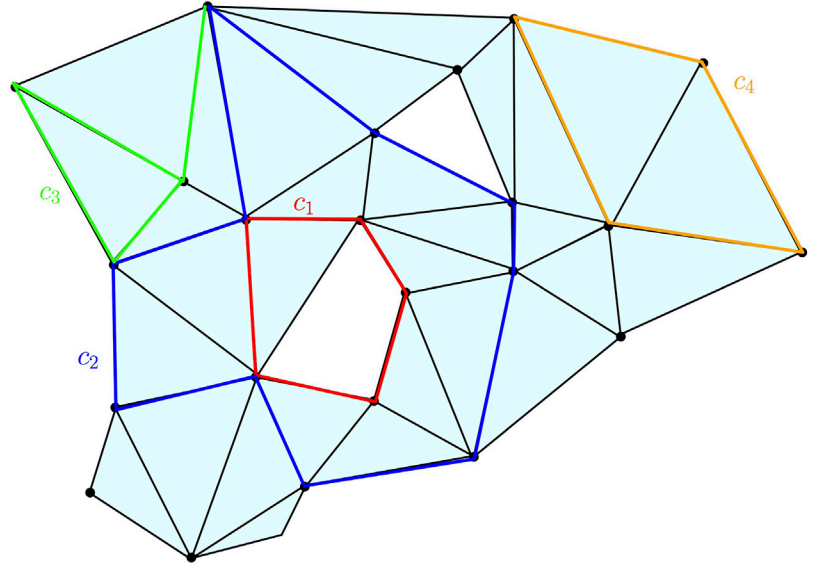
\includegraphics[width=0.85\linewidth]{./figures/Figura6.png}
    \caption{
        Algunos ejemplos de cadenas, ciclos y fronteras en un complejo $K$ de dos dimensiones:
        $c_{1}$, $c_{2}$ y $c_{4}$ son $1$-ciclos; $c_{3}$ es una $1$-cadena pero no un $1$-ciclo;
        $c_{4}$ es una $1$-frontera, la frontera de la $2$-cadena obtenida de la suma de los
        tri\'angulos rodeados por $c_{4}$. Los ciclos $c_{1}$ y $c_{2}$ generan el mismo elemento en
        $H_{1}\left(K\right)$ ya que su diferencia es la $2$-cadena representada por la uni\'on de
        tri\'angulos que rodean la uni\'on de $c_{1}$ y $c_{2}$.
    }
    \label{fig:Figura 6}
    \vspace{15pt}
\end{figure}

Si $c'=\sum_{i=1}^{p}\epsilon_{i}'\sigma_{i}$ es otra $k$-cadena y $\lambda\in\mathbb{Z}_{2}$,
la suma $c+c'$ esta definida como $c+c'=\sum_{i=1}^{p}\left(\epsilon_{i}+\epsilon_{i}'\right)\sigma_{i}$
y el producto $\lambda\cdot c$ esta definido como
$\lambda\cdot c = \sum_{i=1}^{p}\left(\lambda\cdot\epsilon_{i}\right)\sigma_{i}$, convirtiendo a
$C_{k}\left(K\right)$ en un espacio vectorial con coeficientes en $\mathbb{Z}_{2}$. Ya que estamos
considerando los coeficientes en $\mathbb{Z}_{2}$, geom\'etricamente, una $k$-cadena puede ser vista como
una colecci\'on finita de $k$-simplices y la sumas de dos $k$-cadenas como la diferencia sim\'etrica
de las colecciones correspondientes\footnote{Recordemos que la diferencia sim\'etrica entre dos conjuntos
$A$ y $B$ es el conjunto $A\Delta B = \left(A\\B\right)\cup\left(B\\A\right)$}.

La frontera de un $k$-simplejo $\sigma = \left[v_{k},\dots,v_{k}\right]$ es la $\left(k-1\right)$-cadena

\begin{equation*}
    \partial_{k}\left(\sigma\right) = \sum_{i=0}^{k}\left(-1\right)
    \left[v_{0},\dots,\hat{v}_{i},\dots,v_{k}\right]
\end{equation*}

\noindent donde $\left[v_{0},\dots,\hat{v}_{i},\dots,v_{k}\right]$ es el $\left(k-1\right)$-simplejo
generado por todos los v\'ertices a excepci\'on de $v_{i}$\footnote{Ya que estamos considerando
los coeficientes en $\mathbb{Z}_{2}$, se tiene que $-1=1$ y por lo tanto $\left(-1\right)^{i}=1$
para cualquier $i$.}. Dado que los $k$-simplejos forman una base de $C_{k}\left(K\right)$,
$\partial_{k}$ se extiende como una funci\'on lineal de $C_{k}\left(K\right)$ a $C_{k-1}\left(K\right)$
llamado el operador frontera. El kernel de $\partial_{k}$ denotado por: $Z_{k}\left(K\right)=
\left\{c\in C_{k}\left(K\right):\partial_{k}\left(c\right)=0\right\}$ es llamado el espacio de
$k$-ciclos de $K$, y la imagen de $\partial_{k+1}$ denotada por: $B_{k}\left(K\right)=
\left\{c\in C_{k}\left(K\right): \exists c' \in C_{k+1}\left(K\right),
\partial_{k+1}\left(c'\right)=c\right\}$ es llamada el espacio de $k$-fronteras de $K$.

\begin{figure}[ht]
    \centering
    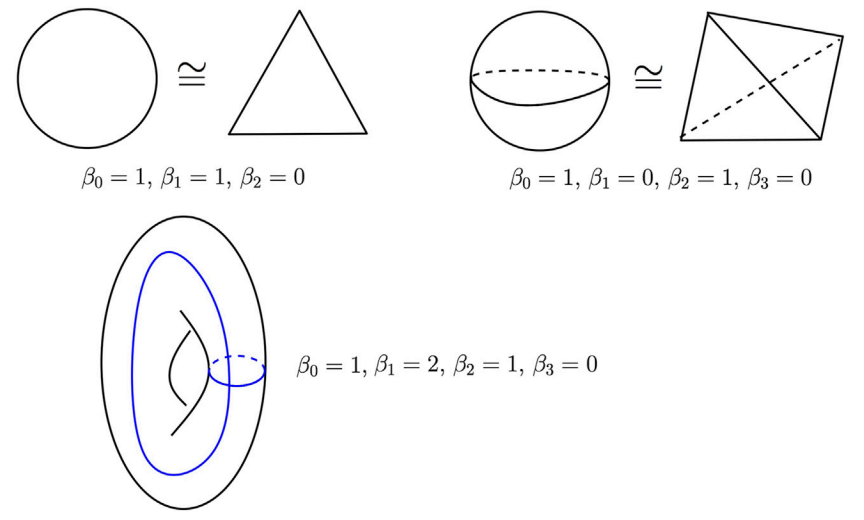
\includegraphics[width=0.85\linewidth]{./figures/Figura7.png}
    \caption{
        N\'umeros de Betti en el c\'irculo, la esfera de dimensi\'on dos y el toro de dimensi\'on dos.
        Las curvas azules en el toro representan dos ciclos independientes cuya clase de homolog\'ia
        es una base para el grupo de homolog\'ia de dimensi\'on uno.
    }
    \label{fig:Figura 7}
    \vspace{15pt}
\end{figure}

\newpage

El operador frontera satisface la siguiente propiedad fundamental:

\begin{equation*}
    \partial_{k+1}\circ\partial_{k+1}\equiv 0 \text{ para cualquier } k\geq 1.
\end{equation*}

\noindent en otras palabras, cualquier $k$-frontera es un $k$-ciclo, esto es,
$B_{k}\left(K\right)\subseteq Z_{k}\left(K\right)\subseteq C_{k}\left(K\right)$. Estas nociones son
ilustradas en la Figura \ref{fig:Figura 6}.

\begin{definicion}
    (grupo de homolog\'ia simplicial y n\'umeros de Betti). El $k$-\'esimo grupo de homolog\'ia
    (simplicial) de $K$ es el espacio cociente
    
    \begin{equation*}
        H_{k}\left(K\right)=Z_{k}\left(K\right)/B_{k}\left(K\right).
    \end{equation*}
    El $k$-\'esimo n\'umero de Betti de $K$ es la dimensi\'on $\beta_{k}\left(K\right)=
    \mathrm{dim}H_{k}\left(K\right)$ del espacio $H_{k}\left(K\right)$.
\end{definicion}

La Figura \ref{fig:Figura 7} muestra los n\'umeros de Betti de algunos espacios sencillos. Dos ciclos,
$c, c' \in Z_{k}\left(K\right)$, se dicen ser hom\'ologos si difieren por una frontera, esto es, si
existe una $\left(k+1\right)$-cadena $d$ tal que $c'=c+\partial_{k+1}\left(d\right)$. Dichos ciclos dan
lugar al mismo elemento de $H_{k}$. En otras palabras, los elementos de $H_{k}\left(K\right)$ son clases
de equivalencia de ciclos hom\'ologos.

Los grupos de homolog\'ia simplicial y los n\'umeros de Betti son invariantes topologicas; si $K$, $K'$
son dos complejos simpliciales tales que sus realizaciones geom\'etricas son homot\'opicamente
equivalentes, entonces sus grupos de homolog\'ia son isomorfos y sus n\'umeros de Betti son iguales.

La homolog\'ia singular es otra noci\'on de homolog\'ia que nos permite considerar una mayor variedad de
espacios topol\'ogicos. Esta definida para cualquier espacio topol\'ogico $X$ de manera similar a la
homolog\'ia simplicial, excepto que el concepto de simplejo, es reemplazado por por el de simplejo
singular, que consiste en una funci\'on continua $\sigma: \Delta_{k}\rightarrow X$ donde $\Delta_{k}$
es el simplejo est\'andar de dimensi\'on $k$. El espacio de las $k$-cadenas es el espacio
vectorial generado por los simplejos singulares $k$-dimensionales, y la frontera de un simplejo $\sigma$
esta definida como la suma (alternante) de la restricci\'on de $\sigma$ a las caras $(k-1)$-dimensionales
de $\Delta_{k}$. Algo importante acerca de la homolog\'ia singular es hecho de que esta coincide con
la homolog\'ia simplicial cuando $X$ es homeomorfo a la realizaci\'on gem\'etrica de un complejo
simplicial. Esto nos permite hablar acerca de la homolog\'ia de un espacio topol\'ogico o un complejo
simplical, sin tener que especificar si nos referimos a la homolog\'ia singular o simplicial.

Observemos que si $f:X\rightarrow Y$ es una funci\'on continua, entonces para cualquier simplejo singular
$\sigma:\Delta_{k}\rightarrow X$ en $X$, se tiene que $f\circ\sigma:\Delta_{k}\rightarrow Y$ es un
simplejo singular en $Y$, de aqu\'i, deducimos que funciones continuas entre espacios topol\'ogicos
inducen homomorfismos entre sus grupos de homolog\'ia. En particular, si $f$ es una equivalencia
homot\'opica, entonces se induce un isomorfismo entre $H_{k}\left(X\right)$ y $H_{k}\left(Y\right)$ para
cualquier $k$ entero no-negativo. Por ejemplo, sea $X\subset \mathbb{R}^{d}$ cualquier conjunto de puntos
y $r>0$, se sigue del teorema del nervio que la $r$-cobertura $X^{r}$ y el complejo de \v Cech
$Cech_{r}\left(X\right)$ tienen grupos de homolog\'ia isomorfos y los mismos n\'umeros de Betti.

%Nuevos comandos

Adem\'as de esto, tenemos como consecuencia del teorema de reconstrucci\'on \ref{teoRecon} el siguiente
resultado que nos auxilia en la estimaci\'on de n\'umeros de Betti.

\begin{teorema}
    Sea $M \subset \mathbb{R}^{d}$ un conjunto compacto con alcance,
    $\mathrm{reach}_{\alpha}\cpar{d_{M}}\geq R > 0$ para alg\'un $\alpha\in\cpar{0, 1}$ y sea $\mathbb{X}$
    un conjunto finito de puntos tales que:
    \begin{equation*}
        d_{H}\cpar{M, \mathbb{R}}=\epsilon < \frac{R}{5+4/\alpha^{2}}.
    \end{equation*}
    Entonces, para cada $r\in\ccorch{4\epsilon/\alpha^{2}, R-3\epsilon}$ y cada $\eta\in\cpar{0, R}$,
    los n\'umeros de Betti de $Cech_{r}\cpar{\mathbb{X}}$ y $M^{\eta}$ son iguales.
    
    En particular, si $M$ es una subvariedad suave de $\mathbb{R}^{d}$ de dimensi\'on $m\in\mathbb{Z}$,
    entonces $\beta_{k}\cpar{Cech_{r}\cpar{\mathbb{R}}}=\beta_{k}\cpar{M}$ para cualquier $k=0, \dots, m$.
\end{teorema}

Desde una perspectiva m\'as pragm\'atica, este resultado nos genera tres problemas: primero, la
suposici\'on de regularidad acerca del $\alpha$-alcance de $M$ puede ser demasiado restrictiva; segundo,
el c\'alculo del nervio de la uni\'on de bolas requiere de m\'etodos para probar que la uni\'on finita de
bolas sea no-vac\'ia; tercero, la estimaci\'on de n\'umeros de Betti recae en la elecci\'on del
par\'ametro $r$.

Para solucionar los problemas anteriores, Chazal y Oudot (2008) \cite{Chazaloudot2008} establecieron el
siguiente resultado que ofrece la soluci\'on a los primeros dos problemas.

\begin{teorema}
    Sea $\mathbb{M}\subseteq\mathbb{R}^{d}$ un conjunto compacto tal que $\mathrm{wfs}\cpar{M}=
    \mathrm{wfs}_{d_{M}}\cpar{0}\geq R>0$ y sea $\mathbb{X}$ un conjunto de puntos finito tal que
    $d_{H}\cpar{M,\mathbb{X}}=\epsilon <\frac{1}{9}\mathrm{wfs}\cpar{M}$. Entonces para cualquier
    $r\in \ccorch{2\epsilon, \frac{1}{4}\cpar{\mathrm{wfs}\cpar{M}-\epsilon}}$ y cualquier
    $\eta\in\cpar{0,R}$,
    \begin{equation*}
        \beta_{k}\cpar{X^{\eta}} = \mathrm{rk}\cpar{H_{k}\cpar{Rips_{r}\cpar{\mathbb{X}}}}
        \rightarrow H_{k}\cpar{Rips_{4r}\cpar{\mathbb{X}}}
    \end{equation*}
    donde $\mathrm{rk}\cpar{H_{k}\cpar{Rips_{r}\cpar{\mathbb{X}}}}
    \rightarrow H_{k}\cpar{Rips_{4r}\cpar{\mathbb{X}}}$ denota el rango de del homomorfismo inducido
    por la inclusi\'on can\'onica (continua)
    $Rips_{r}\cpar{\mathbb{X}}\hookrightarrow Rips_{4r}\cpar{\mathbb{X}}$.
\end{teorema}

Aunque este resultado deja abierta la elecci\'on del par\'ametro $r$, en el estudio realizado por
Chazal y Oudot (2008) \cite{Chazaloudot2008} se provee una descripci\'on de una estrategia multiescala
que ayuda a identificar las escalas relevantes en las cuales se puede aplicar el teorema anterior.

\newpage

\section{Aspectos estad\'isticos de la inferencia homol\'ogica}

De acuerdo a los resultados de estabilidad presentados en la secci\'on anterior, un acercamiento
estad\'istico a la inferencia topol\'ogica se relaciona fuertemente al problema de estimaci\'on de
soportes de distribuciones y estimaciones de conjuntos nivel bajo la m\'etrica de Hausdorff.
Afortunadamente se cuenta con una variedad de metodos y resultados que nos atudan a estimar el soporte de
una distribuci\'on. Por ejemplo, el estimador de Devroye y Wise
(Devroye y Wise 1980 \cite{DevroyeWise1980}) definido en una muestra $\mathbb{X}_{n}$ es tambi\'en una
cobertura  particular de $\mathbb{X}_{n}$. La tasa de convergencia de $\mathbb{X}_{n}$ y el estimador
de Devroye y Wise al soporte de la distribuci\'on para la distancia de Hausdorff fueron estudiados por
Cuevas y Rodriguez-Casal (2004) \cite{CuevasRodriguezCasal2004} en $\mathbb{R}^{d}$. Recientemente, las
tasas de convergencia minimax de estimaci\'on de variedades bajo la metrica de Hausdorff, particularmente
relevantes para la inferencia topol\'ogica, fueron estudiadas por Genovese et al. (2012)
\cite{Genovese2012}. Tambi\'en existe literatura acerca de la estimacion de los conjuntos de nivel en
varias m\'etricas (vease, por ejemplo, Cadre, 2006 \cite{Cadre2006}; Polonik, 1995 \cite{Polonik1995};
Tsybakov, 1997 \cite{Tsybakov1997}) y, particularmente, para la m\'etrica de Hausdorff Chen et al.
(2017) \cite{Chen2017}. Todos estos trabajos acerca de la estimaci\'on de soportes y conjuntos nivel,
dan lugar al an\'alisis estad\'istico de procesos de inferecia topol\'ogica.

En el estudio por Nigoyi et al (2008) \cite{Niyogi2008}, se muestra que el tipo de homotop\'ia de
variedades Riemannianas con alcance mayor que cierta constante puede ser recuperado con una
alta probabilidad de las coberturas de una muestra en (o bien, cerca) de la variedad en cuesti\'on.
Este articulo fue probablemente el primer intento de considerar la inferencia topol\'ogica en t\'erminos
de probabilidad. El estudio por Nigoyi et al.\cite{Niyogi2008} derivo de un argumento de contracci\'on de
retracto y utiliz\'o cotas estrechas sobre el n\'umero de cobertura de la variedad para controlar
la distancia de Hausdorff entre la variedad y la nube de puntos observada. La inferencia homol\'ogica
en el caso de ruido presente, esto es, en el sentido de que la distribuci\'on de la observaci\'on se
concentra alrededor de la variedad, tambi\'en fue estudiado por Nigoyi et al. (2008) \cite{Niyogi2008},
Nigoyi et al. (2011) \cite{Niyogi2008}. La suposici\'on de que el objeto geom\'etrico es una variedad
Riemanniana suave solo es usada en el art\'iculo para controlar la distancia de Hausdorff entre la
muestra y la variedad y no es realmente necesaria para la ``parte topol\'ogica'' del resultado, el cual
es similar a aquellos en los estudios por Chazal et al. (2009) \cite{Chazal2009d}, Chazal y Lieutier
(2008) \cite{Chazal2008} en el entorno particular de las variedades Riemannianas. Empezando por el
resultado del estudio por Nigoyi et al. (2008) \cite{Niyogi2008}, las tasas de convergencia minimax
del tipo de homolog\'ia han sido estudiadas por Balakrishnan et al, (2012) \cite{Balakrishnan2012}
bajo varios modelos de variedades Riemannianas con alcance m\'as grande que cierta constante. En contraste, no se ha propuesto una versi\'on estad\'istica del trabajo por Chazal et al. (2009)
\cite{Chazal2009d}.

M\'as recientemente, siguiendo las ideas encontradas en Nigoyi et al. (2008) \cite{Niyogi2008},
Bobrowski et al (2014) \cite{Bobrowski2014} se ha propuesto un robusto estimador homol\'ogico para los
conjuntos de nivel de funciones de densidad y regresi\'on, por medio de considerar la inclusi\'on entre
pares anidados de conjuntos de nivel estimados obtenidos mediante un estimador del kernel.

\section{M\'as all\'a de la Distancia de Hausdorff: Distancia a una Medida}

Es bien sabido que los m\'etodos del ATD fallan rotundamente en presencia de puntos aislados, a\~{n}adir
un solo punto asilado al conjunto de datos puede alterar la funci\'on distacia de manera dram\'atica
(ver Figura \ref{fig:Figura 8}). Como respuesta a esto, Chazal et al. (2011) \cite{Chazal2011b}
introdujeron una funci\'on distancia alternativa la cual es resistente ante el ruido, la distancia a una
medida.

Dada una distribuci\'on de probabilidad $P$ en $\mathbb{R}^{d}$ y un par\'ametro real $0\leq U\leq 1$,
la noci\'on de distancia al soporte de $P$ puede ser generalizada como la funci\'on

\begin{equation*}
    \delta_{P,u}:x\in\mathbb{R}^{d}\mapsto\inf{t>0:P\cpar{B\cpar{x,t}}\geq u}
\end{equation*}

donde $B\cpar{x,t}$ es la bola cerrada (Euclideana) con centro en $x$ y radio $t$. Para evitar problemas
de discontinuidad con la funci\'on $P\rightarrow \delta_{P,u}$, la funci\'on distancia a la medida (DAM)
con par\'ametro $m\in\ccorch{0,1}$ y potencia $r\geq 1$ esta definida como

\begin{equation}
    d_{P,m,r}\cpar{x}:
    x\in\mathbb{R}^{d}\mapsto\cpar{\frac{1}{m}\int_{0}^{m}\delta_{P,u}^{r}\cpar{x}\,du}^{\frac{1}{r}}
\end{equation}

\par Una propiedad deseable de las DAM demostrada por Chazal et al. (2011)\cite{Chazal2011b} es la
estabilidad con respecto a las perturbaciones de $P$ en la m\'etrica de Wasserstein, m\'as precisamente,
la funci\'on $P\rightarrow d_{P,m,r}$ es $m^{-\frac{1}{r}}$-Lipschitz, esto es, si $P$ y $\tilde{P}$ son
dos distribuciones de probabilidad en $\mathbb{R}^{d}$, entonces

\begin{equation}
    \cnorm{d_{P,m,r}-d_{\tilde{P},m,r}}_{\infty}\leq m^{-\frac{1}{r}}W_{r}\cpar{P,\tilde{P}}
\end{equation}

donde $W_{r}$ es la distancia de Wasserstein para la m\'etrica Euclidiana en $\mathbb{R}^{d}$, con
exponente $r$\footnote{Ver Villiani (2003)\cite{Villiani2003} para la definici\'on de distancia de
Wasserstein}. Esta propiedad implica que la DAM asociada con distribuciones cercanas en la m\'etrica de
Wasserstein tienen conjuntos subnivel cercanos. M\'as a\'un, cuando $r=2$, la funci\'on
$d_{P,m,2}^{2}$ es semiconcava, lo cual asegura fuertes propiedades de regularidad en la
geometr\'ia de sus subniveles. Usando estas propiedades, Chazal et al. (2011) \cite{Chazal2011b} mostr\'o
que bajo suposiciones generales, si $\tilde{P}$ es una distribuci\'on de probabilidad que aproxima a $P$,
as\'i los conjuntos subnivel de $d_{\tilde{P},m,2}$ proveen una aproximaci\'on topol\'ogicamente
correcta al soporte de $P$.

\par En la pr\'actica, la medida $P$ usualmente solo es conocida a trav\'es de un conjunto finito de
observaciones $\mathbb{X}_{n}=\cllav{X_{1},\dots,x_{n}}$ muestreada desde $P$, dando lugar a la pregunta
de una aproximaci\'on a la DAM. Una idea natural para estimar la DAM desde $\mathbb{X}_{n}$ es utilizar
la medida emp\'irica $P_{n}$ en lugar de $P$ en la definici\'on de la DAM. Esto corresponde al computo
de la distancia à la medida emp\'irica (DAME). Para $m=\frac{k}{n}$, la DAME satisface

\begin{equation*}
    d_{P_{n},k/n,r}^{r}\cpar{x}:=\frac{1}{k}\sum_{j=1}^{k}\cnorm{x-\mathbb{X}_{n}}_{\cpar{j}}^{r}
\end{equation*}

donde $\cnorm{x-\mathbb{X}_{n}}_{\cpar{j}}$ denota la distancia entre $x$ y su $j$-\'esima vecindad
en $\cllav{X_{1},\dots,X_{n}}$. Esta cantidad es f\'acil de calcular en la pr\'actica ya que solo
requiere de distancias entre $x$ y los puntos de la muestra. La convergencia de las DAME a las DAM
ha sido estudiada por Chazal et al. (2017)\cite{Chazal2017} y Chazal et al (2016)\cite{Chazal2016b}.

La introducci\'on de las DAM a motivado trabajos y aplicaciones en diferentes direcciones tales como
el an\'lisis topol\'ogico de datos (Buchet et al., 2015\cite{Buchet2015a}), an\'alisis de trazas GPS
(Chazal et al., 2011 \cite{Chazal2011a}), estimaci\'on de densidad (Biau et al., 2011 \cite{Biau2011}),
pruebas de hip\'otesis (Br\'echeteau, 2019 \cite{Brecheteau2019}), y agrupamiento (Chazal et al., 2013
\cite{Chazal2013b}), solo para nombrar algunos. Tambi\'en se han tomado en consideraci\'on,
aproximaciones, generalizaciones, y variantes de las DAM (Guibas et al., 2013 \cite{Guibas2013};
Phillips et al., 2014 \cite{Phillips2014}; Buchet et al., 2015 \cite{Buchet2015b};
Br\'echeteau y Levrard, 2020 \cite{Brecheteau2020}).

\begin{figure}[ht]
    \centering
    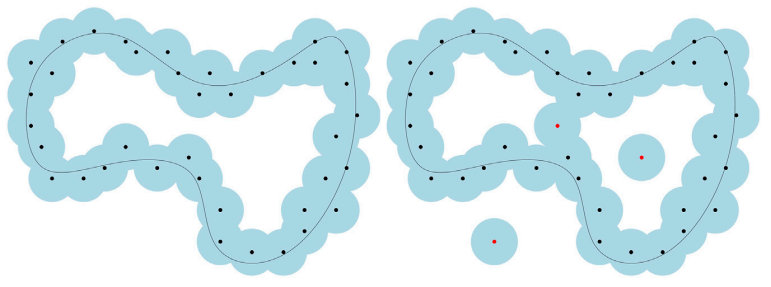
\includegraphics[width=0.85\linewidth]{./figures/Figura8.png}
    \caption{
        Efectos de los puntos aislados en los conjuntos subnivel de las funciones distancia. A\~{n}adir
        unos pocos puntos aislados a la nube puede alterar dram\'aticamente la funci\'on distancia y
        la topolog\'ia de sus coberturas.
    }
    \label{fig:Figura 8}
    \vspace{15pt}
\end{figure}